\documentclass[11pt,a4paper]{article}
\usepackage[margin=2.2cm]{geometry}
\usepackage{graphicx}
\usepackage{booktabs}
\usepackage{float}
\usepackage{caption}
\usepackage[T1]{fontenc}
\usepackage[utf8]{inputenc}

\title{Synthetic Spacing Validation of Voxel-Spacing-Aware PyRadiomics}
\author{}
\date{}

\begin{document}
\maketitle

\section*{Rationale}
This controlled experiment tests software behavior in a synthetic anisotropic image. It compares original PyRadiomics, the modified implementation in default mode, and the modified implementation with \texttt{weightingNorm=voxelSpacing}. The experiment is not a clinical validation study.

\section*{Synthetic Image}
A deterministic 3D image of size $40 \times 40 \times 20$ voxels was generated with a cuboid ROI, a smooth intensity gradient along $x$, alternating bands along $z$, and small fixed-seed noise. Anisotropic spacing was set to $(1.0, 1.0, 5.0)$ in SimpleITK $(x,y,z)$ convention; an isotropic copy used $(1.0,1.0,1.0)$.

\begin{figure}[H]
\centering
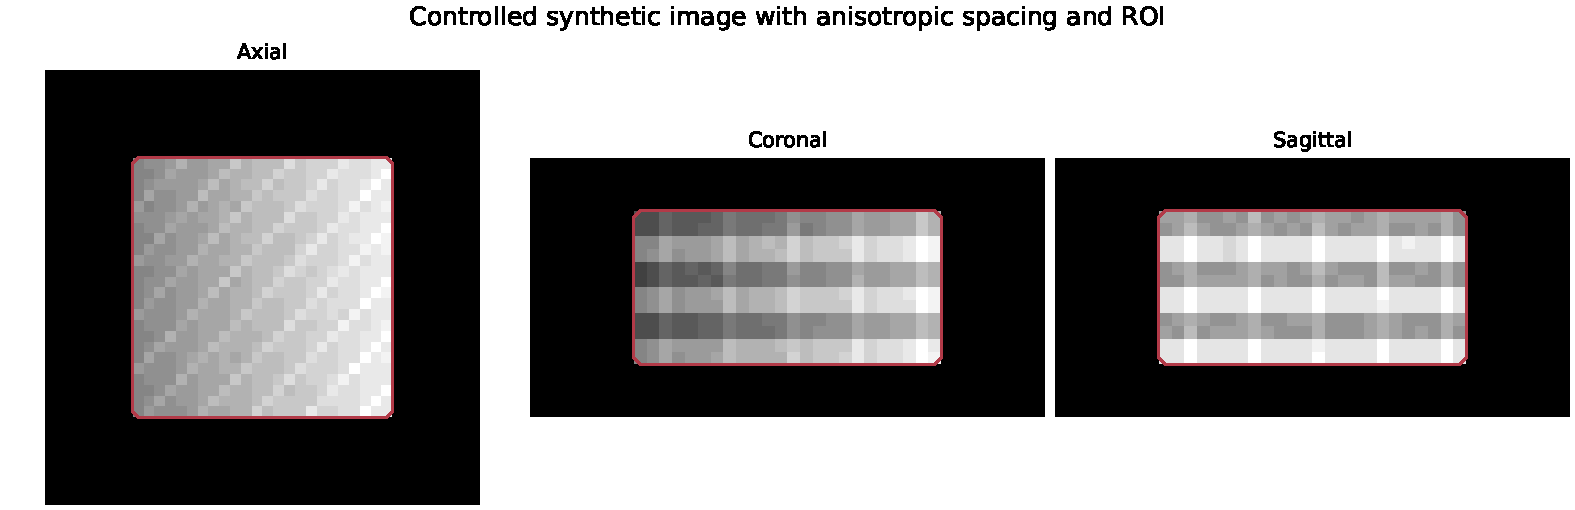
\includegraphics[width=0.92\textwidth]{synthetic_image_slices.pdf}
\caption{Representative slices of the synthetic image with ROI overlay.}
\end{figure}

\section*{Environment Verification}
\begin{tabular}{lllllll}
\toprule
variant & weightingNorm & radiomics & \_cmatrices & \_cshape & spacing & n\_features \\
\midrule
modified\_default\_anisotropic & default & <REPOSITORY_ROOT>/experiments/synthetic\_spacing\_validation/build\_sources/modified/radiomics/\_\_init\_\_.py & <REPOSITORY_ROOT>/experiments/synthetic\_spacing\_validation/build\_sources/modified/radiomics/\_cmatrices.cpython-310-darwin.so & <REPOSITORY_ROOT>/experiments/synthetic\_spacing\_validation/build\_sources/modified/radiomics/\_cshape.cpython-310-darwin.so & [1.0, 1.0, 5.0] & 75 \\
modified\_default\_isotropic & default & <REPOSITORY_ROOT>/experiments/synthetic\_spacing\_validation/build\_sources/modified/radiomics/\_\_init\_\_.py & <REPOSITORY_ROOT>/experiments/synthetic\_spacing\_validation/build\_sources/modified/radiomics/\_cmatrices.cpython-310-darwin.so & <REPOSITORY_ROOT>/experiments/synthetic\_spacing\_validation/build\_sources/modified/radiomics/\_cshape.cpython-310-darwin.so & [1.0, 1.0, 1.0] & 75 \\
modified\_voxelSpacing\_anisotropic & voxelSpacing & <REPOSITORY_ROOT>/experiments/synthetic\_spacing\_validation/build\_sources/modified/radiomics/\_\_init\_\_.py & <REPOSITORY_ROOT>/experiments/synthetic\_spacing\_validation/build\_sources/modified/radiomics/\_cmatrices.cpython-310-darwin.so & <REPOSITORY_ROOT>/experiments/synthetic\_spacing\_validation/build\_sources/modified/radiomics/\_cshape.cpython-310-darwin.so & [1.0, 1.0, 5.0] & 75 \\
modified\_voxelSpacing\_isotropic & voxelSpacing & <REPOSITORY_ROOT>/experiments/synthetic\_spacing\_validation/build\_sources/modified/radiomics/\_\_init\_\_.py & <REPOSITORY_ROOT>/experiments/synthetic\_spacing\_validation/build\_sources/modified/radiomics/\_cmatrices.cpython-310-darwin.so & <REPOSITORY_ROOT>/experiments/synthetic\_spacing\_validation/build\_sources/modified/radiomics/\_cshape.cpython-310-darwin.so & [1.0, 1.0, 1.0] & 75 \\
original\_anisotropic & default & <REPOSITORY_ROOT>/experiments/synthetic\_spacing\_validation/build\_sources/original/radiomics/\_\_init\_\_.py & <REPOSITORY_ROOT>/experiments/synthetic\_spacing\_validation/build\_sources/original/radiomics/\_cmatrices.cpython-310-darwin.so & <REPOSITORY_ROOT>/experiments/synthetic\_spacing\_validation/build\_sources/original/radiomics/\_cshape.cpython-310-darwin.so & [1.0, 1.0, 5.0] & 75 \\
\bottomrule
\end{tabular}


\section*{Backward Compatibility}
\input{table_backward_compatibility.tex}

\section*{Voxel-Spacing Activation}
\begin{tabular}{lllllll}
\toprule
family & n\_features & n\_changed\_strict & n\_changed\_abs\_1e\_5 & median\_abs\_difference & median\_relative\_difference & max\_abs\_difference \\
\midrule
glcm & 24 & 24 & 24 & 0.0958 & 0.101 & 23.3 \\
gldm & 14 & 11 & 11 & 0.118 & 0.491 & 4.73e+03 \\
glrlm & 16 & 16 & 16 & 0.469 & 0.261 & 1.98e+03 \\
glszm & 16 & 8 & 8 & 0.00207 & 0.4 & 1.58e+07 \\
ngtdm & 5 & 5 & 5 & 0.0221 & 0.336 & 9.29 \\
\bottomrule
\end{tabular}


\begin{figure}[H]
\centering
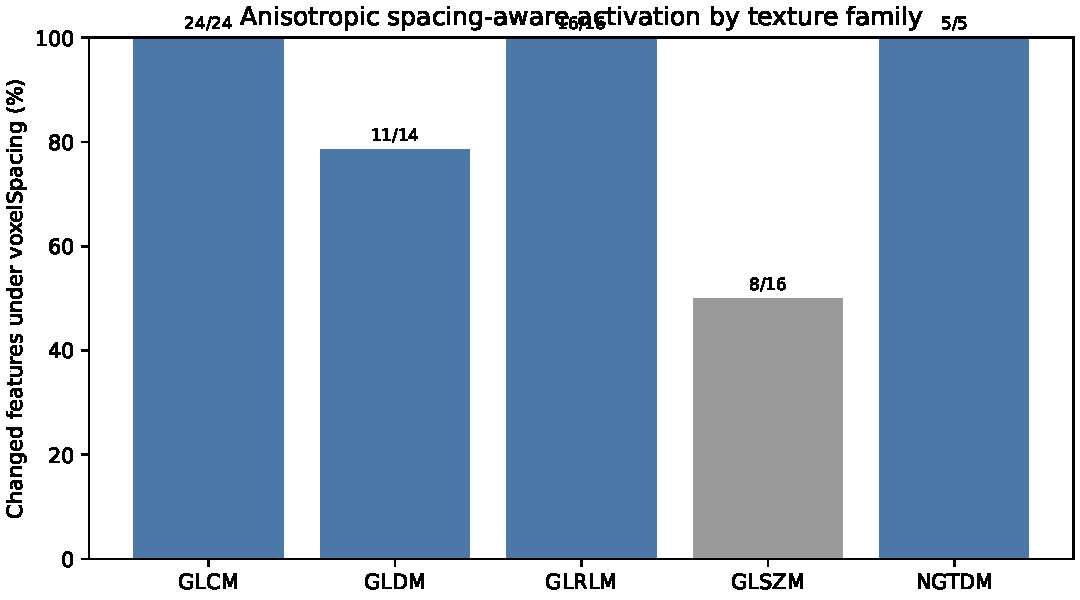
\includegraphics[width=0.78\textwidth]{feature_difference_summary.pdf}
\caption{Percentage of texture features changing after activating voxel-spacing-aware extraction in the anisotropic image.}
\end{figure}

\section*{Isotropic Sanity Check}
\begin{tabular}{llllll}
\toprule
check & n\_features\_compared & mean\_abs\_difference & max\_abs\_difference & n\_changed\_strict & n\_changed\_abs\_1e\_5 \\
\midrule
modified default isotropic vs modified voxelSpacing isotropic & 75 & 0 & 0 & 0 & 0 \\
\bottomrule
\end{tabular}


\section*{Interpretation}
This validation demonstrates software behavior and activation of spacing-aware execution paths under controlled conditions. It does not assess clinical performance. Identical default results between original and modified implementations support backward compatibility. The anisotropic \texttt{voxelSpacing} comparison shows activation of the corrected spacing-aware texture computations, while the isotropic comparison confirms that \texttt{voxelSpacing} now reduces to standard behavior when voxel spacing is equal across axes. This supports the intended implementation principle: spacing-aware extraction should correct anisotropic geometric interpretation without injecting an additional weighting artifact into isotropic data.

\end{document}
